\documentclass[oneside,12pt]{discsthesis}
\usepackage{graphicx}
\usepackage{amsthm}
%\usepackage{multirow}
%\usepackage{fancyvrb}
\usepackage{tabularx}
\usepackage[titletoc]{appendix}
\usepackage{subcaption}
%%\usepackage{rotating}
%%\usepackage{pdfpages}
%\usepackage{lscape}
%\usepackage{adjustbox}
%\usepackage{longtable}
\usepackage{url}
\usepackage{verbatim}

% commands
\newcommand*\diff{\mathop{}\!\mathrm{d}}
\newtheorem{theorem}{Theorem}[chapter]

\title{FinalManuscript_DISCS_UG}
\author{acalab.imagegroup }
\date{March 1, 2018}

\begin{document}

\ThesisAuthor{Aldrich Ellis C. Asuncion \\ Brian Christopher T. Guadalupe}
\ThesisTitle{IMPLEMENTATION AND ANALYSIS OF HOMOMORPHIC FACIAL IMAGE ENCRYPTION AND IMAGE MANIPULATION}
\ThesisArea{Computer Science}
\ThesisDefenseYear{2019}
\DefenseDate{March 1, 2018}


\DepartmentHead{ANDREI D. CORONEL, Ph.D.}
\SchoolHead{EVANGELINE P. BAUTISTA, Ph.D.}
\ThesisAdviser{MARLENE M. DE LEON, Ph.D.}
\FirstPanelMember{MA. MERCEDES T. RODRIGO, Ph.D.}
\SecondPanelMember{JOHN PAUL C. VERGARA, Ph.D.}
\ThirdPanelMember{MA. REGINA JUSTINA E. ESTUAR, Ph.D.}

\ThesisStyle{MS}{Draft}{-10pt}{15pt}

%% Choices for the 1st argument: MS, PhD
%% Choices for the 2nd argument: Final, FinalWithCorner, Draft

%\FrontMatter
% \begin{thesisabstract}
    \noindent
    Homomorphic cryptography allows for encrypted data to be modified and operated on without requiring decryption, although current homomorphic cryptosystems are either limited in their permitted operations or are significantly more time-intensive than standard non-homomorphic cryptosystems. Regardless, homomorphic cryptography has been targeted for use in secure image processing and facial recognition, due to their ability to maintain data privacy. In this paper, we compared the viability of the Paillier, Damg{\aa}rd--Geisler--Kr{\o}igaard (DGK), and Brakerski--Gentry--Vaikuntanathan (BGV) cryptosystems for facial image processing applications, by implementing a software library equipped with these cryptosystems, and comparing their time efficiency and accuracy. Furthermore, as an extension to previous research, we attempt to support non-linear image processing operations by deriving and implementing applicable closed-form approximations. Preliminary results have shown that the Paillier and DGK cryptosystems are comparable in accuracy and may be used for image negation, but only the Paillier cryptosystem is consistent enough to produce reasonable to accurate results.

    % This paper is a sample document that serves as a format and content guideline for undergraduate thesis submissions to the Department of Information Systems and Computer Science. In this section, the abstract, the group should be able to give the readers a clear and concise overview of their study. The section should contain the objectives of the thesis, the methods to be used, and when available, the results of the study, the conclusion, and the recommendations for further work, all based on the intended research objectives. A good abstract should be at most around 150--200 words, or half a page. It should also not contain any references, figures, or equations.
\end{thesisabstract}

% \begin{acknowledgments}

    \noindent
    We would like to thank Dr. Ma. Mercedes Rodrigo, Dr. Ma. Regina Estuar, and Dr. Proceso Fernandez, Jr. for initiating the creation of this thesis template for use of undergraduate thesis groups for years to come. We also extend our gratitude to Ms. Jessica Sugay for help invaluable help in automating many of the formatting of this template, especially in the creation of the custom styles, table of contents, list of figures, list of tables, and the bibliography.

    This section, as the name suggests, is the place in your paper where you may acknowledge individuals or groups who, with their help or guidance, made your study feasible and ultimately a reality. Some of these people include your adviser, volunteers for your study, other professors who may have contributed to your study, and if applicable, any group or organization who provided support in any way for your research.

\end{acknowledgments}

\tableofcontents
\listoffigures
% \listoftables

\MainMatter
\chapter{INTRODUCTION}
 

\section{Context of the Study}

Digital data privacy and security is a growing concern in various fields, such as  cloud computing \cite{potey_homomorphic_2016}, health information systems \cite{kester_cryptographic_2015}, and video surveillance \cite{upmanyu_efficient_2009}. To meet these needs, various cryptosystems have been developed. A cryptosystem is a system which operates on plaintexts, ciphertexts and keys. a cryptosystem also has an encryption algorithm, which maps a plaintext to a ciphertext, and a decryption algorithm, which maps a ciphertext to a plaintext, given an appropiate key \cite[p.119]{tilborg_encyclopedia_2005}. The encryption and decryption algorithms are chosen such that the plaintext cannot easily be recovered from the ciphertext without knowledge of the key. This allows data to be securely transmitted over an insecure channel:  and thus much research has been done on the development and application of various cryptosystems.

One such particular application of cryptography is image encryption. While cryptosystems used to encrypt digital data in general, such as the Advanced Encryption Standard (AES) or elliptic curve cryptography, can also be used to encrypt images \cite{jain_image_2016, singh_image_2015} other algorithms created specifically for image encryption have also been developed \cite{murugan_survey_2018}.

However, research has also considered a type of cryptosystem, homomorphic cryptosystems, where in addition to allowing the secure transmission of data, it is also possible to perform computations with encrypted data, the most basic of which being addition and multiplication. Numerous homomorphic cryptosystems exist, which allow for data to be manipulated without compromising data privacy \cite{fontaine_survey_2007, sen_homomorphic_2013}. In homomorphic image encryption, there is additional interest in being able to perform image manipulation operations on the encrypted data such as image adjustment, filtering, and morphological/feature extraction operations \cite{ziad_cryptoimg:_2016, gonzalez_digital_2008}.

\section{Research Objectives}

A paper published in 2009 by Ziad, et. al. presents \textit{CryptoImg}, a library for the  Open Source Computer Vision Library (OpenCV) \cite{opencv_library} which implements various homomorphic encryption and image processing routines using the Paillier homomorphic cryptosystem \cite{ziad_cryptoimg:_2016}. While \textit{CryptoImg} demonstrates that various image manipulation operations are possible in a homomorphic system, we believe this study can be extended by considering other known homomorphic encryption schemes, such as an elliptic curve and ElGamal based cryptosystem presented by Li, et. al. \cite{li_elliptic_2012}, and the fully homomorphic encryption scheme proposed by Smart and Vercauteren \cite{hutchison_fully_2010}. Our study aims to provide an objective comparision of various homomorphic cryptosystems currently in the literature, as they would be used in encrypted image manipulation.
Furthermore, one of the main problems in homomorphic encryption is the practicality of homomorphic encryption schemes. Homomorphic cryptosystems are known to be slower compared to other cryptosystems \cite{sen_homomorphic_2013}.
Taking the above into account, in this study, we wish to
\begin{enumerate}
    \item Compare the applicability of known homomorphic encryption schemes to common image processsing operations, in other words, determine which schemes permit more image processing operations;
		\item Compare the security of common image processsing operations under known homomorphic encryption schemes, using established statistical methods in image encryption;
    \item Compare the efficiency of common image processsing operations under known homomorphic encryption schemes;
    \item Create a plug-in for OpenCV to allow for convenient use of these homomorphic encryption schemes.
\end{enumerate}

\section{Research Questions}

By implementing homomorphic cryptosystems and creating an OpenCV library so they can be easily used, we aim to address our main research question: What is the best method for image data to be encrypted and manipulated for practical applications?

More specifically, our research will address the following sub-questions:
\begin{enumerate}
	\item Which homomorphic cryptosystems admit more image processing operations? How can existing homomorphic cryptosystems be modified to admit more image processing operations?
	\item Which homomorphic cryptosystems are the most time-efficient in applying image processing operations?
	\item Which homomorphic cryptosystems best preserve image quality in applying image processing operations?
\end{enumerate}

\section{Scope and Limitations of the Study}
Our study will be limited in terms of the cryptosystems to be tested, the image processing operations we will implement, and the statistical tests we will use to gauge the security of the cryptosystems. Below is a listing of the scope of the study.

\subsection{Scope of Testing}
We will implement and test the following algorithms:
\begin{enumerate}
	\item A modified version of the Paillier cryptosystem \cite{} which supports floating-point operations, used in \textit{CryptoImg} \cite{ziad_cryptoimg:_2016}.
	\item An elliptic curve and ElGamal based cryptosystem for homomorphic encryption presented by Li, et. al. \cite{li_elliptic_2012}.
	\item A fully homomorphic encryption scheme proposed by Smart and Vercauteren \cite{hutchison_fully_2010}, which is an improvement on the original lattice-based cryptosystem presented by Gentry \cite{gentry_fully_2009}.
\end{enumerate}
We will implement and test the following categories of image manipulation operations:
\begin{enumerate}
	\item Image adjustment
	\item Operations based on convolution
	\item Morphological operations
\end{enumerate}
We will adopt the benchmark for evaluating the performance and security of image encryption schemes presented by Ahmed, et. al \cite{ahmed_benchmark_2016}. The presented benchmark reflects many tests used in other literature \cite{ahmad_efficiency_2012, wu_npcr_2011}.
\begin{enumerate}
	\item Tests for preservation of image quality after encryption and decryption.
	\begin{enumerate}
		\item Mean Squared Error (MSE)
		\item Peak Signal to Noise Ratio (PSNR)
		\item Structural Similarity Index (SSIM)
		\item Noise tolerance
	\end{enumerate}
	\item Tests for cryptographic security
	\begin{enumerate}
		\item Information entropy analysis
		\item Correlation coefficient analysis
		\item Differential analysis (number of pixel change rate (NPCR), universeral average change intensity (UACI))
	\end{enumerate}
\end{enumerate}
A detailed overview of the above will be provided in the review of related literature.

Images used for testing will be obtained from a database maintained by Gonzalez, et. al. \cite{gonzalez_image_nodate}. Both greyscale and color images will be used.

\subsection{Scope of Implementation}
Our library for OpenCV will be implemented in the C++ programming language.

\section{Significance of the Study}


If the Research Objective answers the ‘what’ of your study, this section aims to answer the ‘why’. Generally, you may address this significance in terms of its significance in the area of Computer Science and the community. However, other questions which you may also use to guide your significance are the following: “Why is your study important?” “What will your study contribute to the field of Computer Science?” “How will your study benefit not only your intended audience, but the general public, especially our country?”

\chapter{REVIEW OF RELATED LITERATURE}

\section{Homomorphic Cryptosystems}
% [include mention of metrics by which they are compared]

In cryptography, a cryptosystem consists of an encryption function $\mathcal{E}$ and a decryption function $\mathcal{D}$, along with the plaintext space $\mathcal{P}$, ciphertext space $\mathcal{C}$ and the key space $\mathcal{K}$~\cite{bauer_cryptosystem_2005}. A \textit{plaintext} is text that can be easily understood by everybody. On the other hand, a \textit{ciphertext} is a result from encrypting the plaintext using an encryption key. The \textit{plaintext space} is the set of all possible plaintexts, the \textit{ciphertext space} is the set of all possible ciphertexts, while the \textit{keyspace} consists of all possible keys.

There are two kinds of cryptosystems, namely: \textit{symmetric} and \textit{asymmetric}. In symmetric-key cryptosystems, the same key is used for both encryption and decryption. As a consequence, the encryption and decryption functions are inverses of each other. Prominent examples of symmetric-key cryptosystems are the Data Encryption Standard (DES), and its replacement, the Advanced Encryption Standard (AES).

On the other hand, asymmetric-key (or public-key) cryptosystems use separate keys for encryption and decryption. The encryption key (also called the \textit{public key}) is shared to everybody, while the decryption key (also called the \textit{private key}) is kept secret. Because of this, there is no need to agree upon some secure key sharing protocols. Usually, the security of asymmetric-key cryptosystems relies on the intractability of certain computational problems, like how RSA depends on the difficulty of integer factorization \cite{rivest_method_1978}, while ElGamal depends on the difficulty of the discrete logarithm problem \cite{blakley_public_1985}.

Homomorphic cryptosystems are a special type of cryptosystem wherein operations can be securely performed on encrypted data. Suppose that for a public-key cryptosystem, $\mathcal{E}_k \left(p \right)$ is the encryption function using the public key $k \in \mathcal{K}$, and $\mathcal{D}_l \left(c \right)$ be the decryption function using the private key $l$. A cryptosystem is said to be homomorphic if its encryption function is homomorphic, that is, if it satisfies the relation
\begin{equation}
    \mathcal{E}_k \left(p_1 \boxplus p_2\right) = \mathcal{E}_k \left(p_1\right) \oplus \mathcal{E}_k \left(p_2\right)
\end{equation}
where $p_1, p_2 \in \mathcal{P}$ are the plaintexts, and $\boxplus$ and $\oplus$ are operations in $\mathcal{P}$ and $\mathcal{C}$ respectively \cite{fontaine_survey_2007}. Furthermore, a homomorphic cryptosystem also satisfies \cite{li_elliptic_2012}
\begin{equation}
    p_1 \boxplus p_2 = \mathcal{D}_l \left( \mathcal{E}_k \left(p_1\right) \oplus \mathcal{E}_k \left(p_2\right) \right).
\end{equation}
In other words, a homomorphic cryptosystem preserves the operations that can be typically done with the plaintext without the intermediary step of decrypting the ciphertext beforehand. An important note about the defintion of a homomorphic cryptosystem is that the operations $\boxplus$ and $\oplus$ need not be the same. A simple operation in the plaintext space may require a computationally intensive operation in the ciphertext space.

Some examples of homomorphic cryptosystems include the Goldwasser-Micali cryptosystem \cite{goldwasser_probabilistic_1984} and the Paillier cryptosystem \cite{stern_public-key_1999}. Even the classic public-key cryptosystems are homomorphic, both RSA and ElGamal are multiplicatively homomorphic, while elliptic curve cryptosystems are additively homomorphic \cite{li_elliptic_2012}.

However, there exists a \textit{fully homomorphic} cryptosystem, where instead of being limited to operations like addition or multiplication, it allows any arbitrary operations on the ciphertext. It is only in recent years that a fully homomorphic cryptosystem has been described. Gentry's cryptosystem, which uses lattice-based cryptography, allows arbitrary functions that are constructed from various addition and multiplication operations \cite{gentry_fully_2009}.

A recent survey of homomorphic encryption by Sen shows that the open problems in the area deal with fully homomorphic encryption, of which the main concern is the speed of such implementations \cite{sen_homomorphic_2013}.


\section{Common Image Operations}
% skim chapters 3-4 of the book Digital Image Processing

% we may refer to the classification in the CryptoImg paper
Knowing that most of the common image operations rely on addition and multiplication operations, adopting a fully homomorphic cryptosystem enables image processing operations on encrypted images without the need of decryption.

In image processing, the typical image operations being done are intensity transformations which maps intensity values to another, and the use of spatial filters to do operations such as edge detection and image blurring.

\subsection{Intensity Transformation}
Intensity transformations are typically point operations, where a certain operation is applied to each single pixel of the image. Usually, there is a function $T$ that maps a pixel value $r$ into a new value $r^\prime$, thus this transformation satisfies the relation $r^\prime = T\left(r\right)$. Examples of intensity transformations are image negation, log transformation, and power-law transformation.

Image negation is an example of an intensity transformation, where the resulting image would be similar to a photographic negative~\cite{gonzalez_digital_2008}. In this case, suppose the intensity levels of an image are within the range $\left[0, L-1\right]$, then image negation can be expressed by
\begin{equation}
    T\left(r\right) = L-1-r
\end{equation}

The log transformation is used to enhance dark pixels or increase the dark details of an image by mapping low intensity values to a wider range of values~\cite{gonzalez_digital_2008}. This has the general form
\begin{equation}
    T\left(r\right) = c \log\left(1 + r\right)
\end{equation}
where $c$ is a constant and $r \ge 0$.

The power-law transformation is a family of transformations that have the form
\begin{equation}
    T\left(r\right) = c r^{\gamma}
\end{equation}
where $c>0$ and $\gamma > 0$. This is especially useful since many output devices such as printers and display devices follow the power law, and so correcting the power-law response on these devices in a process called \textit{gamma correction} ensures reproducibility and accuracy of images being displayed~\cite{gonzalez_digital_2008}.

\subsection{Edge Detection and Spatial Filtering}
Edge detection is used to find and determine the boundaries in an image, commonly used in applications such as image segmentation and feature extraction. This works by detecting so-called \textit{edges}, areas that have abrupt changes in intensity.

Edge detection is usually done by using gradient operators that detect such abrupt changes. These operators are commonly known as \textit{spatial filter}, which are usually of $3 \times 3$ size. A common example of spatial filters is the Sobel operator, with two matrices (also called as kernels) $g_x$ and $g_y$ representing the horizontal and vertical components respectively.
\begin{equation}
    g_x =
    \begin{bmatrix}
        -1 & 0 & 1 \\
        -2 & 0 & 2 \\
        -1 & 0 & 1
    \end{bmatrix}
    \qquad\text{and}\qquad
    g_y =
    \begin{bmatrix}
        1 & 2 & 1 \\
        0 & 0 & 0 \\
        -1 & -2 & -1
    \end{bmatrix}
\end{equation}
To get the resulting image $I^\prime$, a convolution is performed between the original image $I$ of size $M \times N$ and the kernel $k$ of size $m \times n$. Now suppose that the pixel value of an image at point $\left(i,j\right)$ is $r_{i,j}$. Then, a transformation using spatial filters can be described as follows:
\begin{align}
    T\left(r_{i,j}\right) &= \left[k * I\right]\left(\left\lfloor\frac{m}{2}\right\rfloor, \left\lfloor\frac{n}{2}\right\rfloor \right) \\
                         &= \sum_{u=1}^{m} \sum_{v=1}^{n} \left[k_{i,j} r_{i+u, j+v} \right]
\end{align}

Spatial filters are not only used for edge detection, but there are also filters that do image smoothing (such as Gaussian blur and box blur, $b_g$ and $b$ respectively in Equation~\ref{eqn:smooth-filters}) and image sharpening, to name a few \cite{gonzalez_digital_2008}.
\begin{equation}
    \label{eqn:smooth-filters}
    b_g = \frac{1}{16}
    \begin{bmatrix}
        1 & 2 & 1 \\
        2 & 4 & 2 \\
        1 & 2 & 1
    \end{bmatrix}
    \qquad
    b = \frac{1}{9}
    \begin{bmatrix}
        1 & 1 & 1 \\
        1 & 1 & 1 \\
        1 & 1 & 1
    \end{bmatrix}
\end{equation}
% Should I put a table of other kernels too?


\section{Related Work and Previous Implementations}
% CryptoImg

% example of homomorphic encryption / image manipulation past work

% minor limitation: improvement on previous work, but not a direct comparison

% major limitation: does not discuss security: are modified images also secure?

There has been work done regarding the application of homomorphic cryptosystems in image processing. In particular, Ziad, et al. introduced a library called \textit{CryptoImg} that uses the homomorphic properties of the Paillier cryptosystem to apply image operations securely \cite{ziad_cryptoimg:_2016}. This shows that it is indeed possible to do various image operations in a homomorphic cryptosystem.

However, a major limitation of \textit{CryptoImg} is that it does not seem to tackle the problem of security. Even though the authors claim that the operations in \textit{CryptoImg} are privacy-preserving, it is not clear whether the modified images are secure as well.
This study can be further improved by also considering the use of other homomorphic cryptosystems like the elliptic curve-based ElGamal cryptosystem by Li, et al. \cite{li_elliptic_2012} and a fully homomorphic cryptosystem introduced by Smart and Vercauteren \cite{hutchison_fully_2010}, which is a variant of Gentry's lattice-based cryptosystem.

% HElib
Another related work would be the implementation of a fully homomorphic encryption. Halevi and Shoup \cite{garay_algorithms_2014} introduced \textit{HElib}, a library that implements the Brakerski-Gentry-Vaikuntanathan (BGV) homomorphic cryptosystem. This library also makes use of various optimizations to speed up the homomorphic operations, due to homomorphic cryptosystems being slower than other cryptosystems \cite{sen_homomorphic_2013}.


\section{Summary}
We have seen how various image processing operations make use of a series of additions and multiplications. Because of this, it is possible to use a homomorphic cryptosystem in order to apply image operations directly on encrypted images, as demonstrated by the \textit{CryptoImg} library.

In particular, we aim to address the shortcoming of \textit{CryptoImg} by developing a library to test various homomorphic encryption schemes with the help of the \textit{HElib} library to be able to implement fully homomorphic encryption schemes. This helps us determine the practicality of using homomorphic cryptosystems in image processing, especially when dealing with more complex image operations.

\chapter{METHODOLOGY}

The study consists of two parts: first, the implementation of the three homomorphic encryption schemes~\cite{ziad_cryptoimg:_2016, dasgupta_design_2016, hutchison_fully_2010} and image processing operations under each scheme as an OpenCV library. While the scheme in~\cite{ziad_cryptoimg:_2016} has been implemented for use in image processing, the fully homomorphic systems~\cite{dasgupta_design_2016, hutchison_fully_2010} will have to be adapted for image processing. The second part of the study consists of assessing the robustness and security of image operations under each encryption scheme using benchmarks in~\cite{ahmed_benchmark_2016}.

\section{Implementation of the OpenCV Library}

The current version of the OpenCV library (3.4.2) will be forked from the open-source GitHub repository at \url{https://github.com/opencv/opencv}~\cite{bradski_opencv_2000}.

Three homomorphic encryption schemes will be implemented, those presented by Ziad, et al.~\cite{ziad_cryptoimg:_2016}, Dasgupta and Pal~\cite{dasgupta_design_2016} and Smart and Vercauteren~\cite{hutchison_fully_2010}. The encryption and decryption methods will be implemented in Python. However, these methods will be also implemented in C++ if time permits. 

Aside from implementing the homomorphic encryption and decryption algorithms, we will also implement library functions for the following image processing functions, as they are defined in~\cite{gonzalez_digital_2008}. We will also take note of whether or not a candidate operation is impossible to perform under a given cryptosystem.  We let $R(x,y)$ denote the intensity at coordinate $(x,y)$ in the source image, and $S(x,y)$ denote the intensity at coordinate $(x,y)$ in the resulting image. We further suppose that the intensity values of pixels are in the range $[0, L-1]$.
\begin{description}
	\item[Intensity transformations.] Transformations on the intensities of each of the pixels on an image. The following definitions hold for all $x,y$.
	\begin{enumerate}
		\item Image negation: $S(x,y) = L - 1 - R(x,y)$.
		\item Log transformation: $S(x,y) = c\log{(1 + R(x,y))}$, $c \geq 0$.
		\item Power-law transformation: $S(x,y) = c[R(x,y)]^\gamma$, $c > 0, \gamma > 0$.
	\end{enumerate}
	\item[Spatial filters.] Filters implemented by performing a convolution between an $M\times N$ source image and an $m\times n$ filter matrix. Let $W$ be a filter matrix. Then the corresponding spatial filter is given by
	\begin{align}
		S(x,y) = \sum_{s=1}^m{\sum_{t=1}^n{W(s,t)R(x+s,y+t)}}.
	\end{align}
	Morphological operations such as erosion and dilation can be achieved using convolution as well.
\end{description}

\section{Assessment of Homomorphic Encryption Schemes}

We will first obtain standard test images from~\cite{gonzalez_image_nodate}. Both grayscale and color images will be used.

For each plaintext image (PT), we will consider each image operation listed above and generate three images: a plaintext domain transformation (PDT), a ciphertext image (CT), and an encrypted domain transformation (EDT). The PDT will be generated by running the image operation on the original image. The CT will be generated by encrypting the image, then applying the operation, and the EDT will be generated by decrypting the CT. The four images (PT, PDT, CT, CDT) will then be compared using various benchmarks to evaluate the quality and security of each homomorphic encryption scheme.

Lab computers in Faura Hall, Ateneo de Manila University will be used to perform the computations, and processing time will be tracked using built-in timing functions.
The processing time for all cases will be recorded.

\subsection{Evaluating Image Quality}
The benchmarks to be used in the study, adopted from~\cite{ahmed_benchmark_2016, ahmad_efficiency_2012, wu_npcr_2011} are listed below. We let $X_i$ denote a value in an image $X$, where $1 \leq i \leq N$.
We first perform three tests to ascertain the preservation of image quality after encryption and decryption: MSE, PSNR, and SSIM.
\begin{description}
	\item [Mean Squared Error (MSE).] The MSE is defined in~\cite{ahmed_benchmark_2016} as
	\begin{align}
        \mathrm{MSE} = \frac{1}{N}\sum_{i=1}^{N}{(\mathrm{CDT}_i - \mathrm{PDT}_i)^2}.
	\end{align}
	The MSE provides a measure of how much data is recovered if an image operation is applied on the encrypted image, which is then decrypted. Lower values of MSE indicate higher preservation of image quality~\cite{ahmed_benchmark_2016, ahmad_efficiency_2012}.
	\item [Peak Signal to Noise Ratio (PSNR).]
	According to Ahmed, et al.~\cite{ahmed_benchmark_2016}, PSNR is ``an estimator for human visual perception of reconstruction quality.'' It has been used to ascertain image quality in various studies and is a known metric for image and video quality~\cite{upmanyu_efficient_2009, jain_image_2016, akramullah_video_2014}. Although it may produce results which do not correlate with human visual perception~\cite{huynh-thu_accuracy_2012, ahmed_benchmark_2016}, it is a valid indicator of image quality when media containing the same visual content is compared~\cite{huynh-thu_accuracy_2012}.
	PSNR is defined by
	\begin{align}
        \mathrm{PSNR} = 10\log_{10}{\left( \frac{L^2}{\mathrm{MSE}} \right)}
	\end{align}
	where $L$ is the maximum pixel intensity value of an image.
	Despite the known limitations of PSNR, since we are going to compare the effect of each encryption scheme on recovered image quality, given a fixed library of images, it is a valid measure of image quality for the study. A higher PSNR indicates higher image quality preservation.
	\item [Structural Similarity Index (SSIM).]
	The SSIM for two random variables $X$ and $Y$ is defined in~\cite{ahmed_benchmark_2016, akramullah_video_2014} as
	\begin{align}
        \mathrm{SSIM}(X,Y) = \frac{(2\mu_X\mu_Y+c_1)(2\sigma_{XY}+c_2)}{(\mu_X^2+\mu_Y^2+c_1)(\mu_X^2+\mu_Y^2+c_2)}
	\end{align}
	where
	\begin{itemize}
		\item $\mu_X, \mu_Y$ are the averages of $X$ and $Y$, respectively;
		\item $\sigma_X, \sigma_Y$ are the variances of $X$ and $Y$, respectively;
		\item $\sigma_{XY}$ is the covariance of $X$ and $Y$;
		\item $c_1 = (k_1L)^2, c_2 = (k_2L)^2$ are two variables used to stabilize the measure when $\mu_X^2+\mu_Y^2$ is close to zero~\cite{akramullah_video_2014};
		\item $L$ is the the maximum pixel intensity value of an image;
		\item $k_1 = 0.01, k_2 = 0.03$ by default, given in~\cite{ahmed_benchmark_2016}.
	\end{itemize}
	The SSIM is applied to the luminance value of two images to gauge structural similarity between neighboring pixels.
    For the study, we will compute $\mathrm{SSIM}(\mathrm{PDT}, \mathrm{CDT})$ for every image operation, under each homomorphic cryptosystem. Higher values of SSIM indicate higher structural similarity, and an SSIM of $1$ indicates that the two images are identical~\cite{ahmed_benchmark_2016}.
\end{description}

\subsection{Evaluating Cryptographic Security}
After performing tests to evaluate image quality, we then perform tests for cryptographic security, as enumerated in~\cite{ahmed_benchmark_2016}: entropy analysis, correlation coefficient analysis (CC), NPCR and UACI.
\begin{description}
	\item [Information entropy analysis.] In information theory, the entropy function $H(X)$ is defined in~\cite{bauer_information_2005} as
	\begin{align}
		H(X) = - \sum_{a:p_X(a)>0}{p_X(a)\log_2{p_X(a)}}
	\end{align}
	where $p_X(a)$ denotes the probability that the random variable $X$ takes on the value $a$.
	In the analysis of image encryption, $H(X)$ is computed for the values of the ciphertext pixels. To ensure security against entropy attacks, $H(X)$ must be as close as possible to $\log_2{N}$, where $N$ is the number of possible pixel values~\cite{ahmed_benchmark_2016}.

    We will compute $H(\mathrm{CDT})$ for every image operation, under each homomorphic cryptosystem, and compare the effects of each image operation on the entropy of the encrypted image. Ideally, performing image operations on encrypted images should still maintain a high level of entropy.
	\item [Correlation coefficient analysis (CC).]
		Images generally have a high degree of similarity between adjacent pixels. This correlation must be hidden in the encrypted image, even after performing image operations.
		The correlation coefficient of an image can be computed between adjacent pixels either vertically, horizontal, or diagonally, and is defined in~\cite{ahmed_benchmark_2016} by:
		\begin{align}
            \mathrm{CC}(X,Y) = \frac{\sigma_{X,Y}}{\sqrt{\sigma_X}\times\sqrt{\sigma_Y}}
		\end{align}
		where
		\begin{itemize}
			\item $\sigma_X, \sigma_Y$ are the variances of $X$ and $Y$, respectively;
			\item $\sigma_{XY}$ is the covariance of $X$ and $Y$.
		\end{itemize}

        For every $\mathrm{CDT}$ image, we will compute for the correlation coefficient (for vertical, horizontal and diagonal correlation) for every image operation, under each homomorphic cryptosystem.
	\item [NPCR and UACI.]
		The Number of Pixel Change Rate (NPCR) measures the number of pixels which are changed between the a plaintext and a ciphertext to quantify the amount of dispersion which occurs during encryption.

		On the other hand, the Universal Average Change Intensity (UACI) measures the average difference in pixel intensity between two images.

		The NPCR and UACI between two images $X$ and $Y$, each containing $N$ pixels indexed from $1$ to $N$ is defined in~\cite{wu_npcr_2011} as
		\begin{align}
            \mathrm{NPCR}(X,Y) &= \frac{1}{N}\sum_{i = 1}^{N}{D(X_i,Y_i)} \times 100\%\\
            \mathrm{UACI}(X,Y) &= \frac{1}{L_{\max} \times N} \sum_{i = 1}^{N}{ |L(X_i) - L(Y_i)| } \times 100\%
		\end{align}
		where
		\begin{itemize}
			\item $X_i$ and $Y_i$ are the $i$th pixels of $X$ and $Y$, respectively;
			\item $D$ is a difference function between pixels $A$ and $B$ defined by
			\begin{align}
				D(A,B) =
				\begin{cases}
					0 &  \text{if $A = B$},\\
					1 &  \text{if $A \neq B$};
				\end{cases}
			\end{align}
		\item $L_{\max}$ is the maximum intensity of a pixel;
		\item $L(X_i)$ and $L(Y_i)$ are the intensities of pixels $X_i$ and $Y_i$, respectively.
		\end{itemize}
        We will calculate $\mathrm{NPCR}(\mathrm{PDT},\mathrm{CDT})$ and $\mathrm{UACI}(\mathrm{PDT},\mathrm{CDT})$  for every image operation, under each homomorphic cryptosystem. A high NPCR and UACI are desired to ensure high dispersion and security against differential attacks~\cite{ahmed_benchmark_2016}. Critical values for NPCR and UACI for given image sizes and bit depths are given in~\cite{wu_npcr_2011}.
\end{description}

\section{Summary}

In summary, the study will consist of
\begin{itemize}
	\item An implementation of an OpenCV library which implements homomorphic cryptosystems by Ziad, et al.~\cite{ziad_cryptoimg:_2016}, Dasgupta and Pal~\cite{dasgupta_design_2016} and Smart and Vercauteren~\cite{hutchison_fully_2010}.
	\item An implementation of image processing operations (intensity transformations, spatial filters) under the above cryptosystems.
	\item Conducting tests for image quality, processing time, and cryptographic security, using standard test images from~\cite{gonzalez_image_nodate}.
\end{itemize}

These will be conducted over the course of the first semester of AY 2018--2019 to allow for analysis of the results and paper preparation in the second semester. Additional cryptosystems, image operations, and cryptographic security tests may be included in the scope of the study, depending on future research.

We now provide a summary of how each of our reserch questions are addressed by the methodology.
\begin{itemize}
	\item \textbf{Applicablity of homomorphic encryption algorithms for the use of image processing operations on encrypted data?} This will be addressed by the implementation of OpenCV library, and the evaluation of image quality (MSE, PSNR, SSIM).
	\item \textbf{Time efficiency in applying image manipulation operations.} This will be addressed by the implementation of OpenCV library, and the comparison of recorded processing time for image processing operations.
	\item \textbf{Security under differential and entropy attacks.}
	This will be addressed by the evaluation of security benchmarks for image encryption schemes (entropy analysis, correlation coefficient analysis, NPCR, UACI).
\end{itemize}

% \chapter{RESULTS AND DISCUSSION}
After implementing your methodology and gathering all pertinent data, in this section, you will now present the gathered data to your reader. By the end of this section, your reader should have an idea of what exactlty happened during the experiment. 
A good way to organize your results is to group them is to present them in the same order which your methodology was presented. For instance, if your methodology included the analysis of user logs, the implementation of an application, and the testing of this application, your results should flow in the same way. In addition, more often than not, you will be presenting a large volume of data, so utilize figures and tables whenever appropriate. Table 5.1 below presents one way of how to go about presenting your data. Note the table caption and headers, as mentioned in our framework.


\begin{table}[t]
\centering
\caption {Preliminary Test Result, organized by Problem Type}
\label{tab:acc_lit} 
\begin{tabular}{ c  c  c  c  c  c  c  c  c  c  c }
\hline
Problem	&Average 	&Standard 	&Average 		&Standard		&Dominant\\
Type  &Steps   &Deviation   &Duration   &Deviation   &Affective\\
  &   &(Steps)   &(s)   &(Duration)   &State\\ \hline

A1  &14   &2.30   &23.04   &3.50   &CONF\\
A2  &2   &5.36   &32.10   &2.01   &FLOW\\
A3  &31   &1.01   &28.55   &4.03   &FLOW\\
B1  &24   &4.40   &45.30   &3.30   &BOR\\
B2  &33   &2.12   &20.56   &2.21   &FLOW\\
B3  &36   &1.05   &LOSE   &1.15   &CONF\\
C1  &22   &1.33   &LOSE   &1.40   &FLOW\\
C2  &23   &3.03   &LOSE   &1.30   &FLOW\\
D1  &30   &1.79   &LOSE   &1.45   &FLOW\\
D2  &15   &1.30   &LOSE   &1.05   &FLOW\\ \hline
\end{tabular}
\end{table}


There are, however, some additional notes that must be clarified. First, given that you will be gathering a huge volume of data, you must be able to classify which of these were critical in determining the outcome of your study, and which ones need not be presented. The critical data must be presented in this section, while the minor ones may be placed in the Appendices of your paper, which will be described later in this template.

Another clarification to be noted is that the presentation of results in this section must be objective, or `as-is'. This means that you must describe your results in a way understandable to your reader without putting any form of interpretation. In effect, this section’s intent is to provide answers to ``what happened'' questions, not ``what does it mean'' questions. The interpretation of results is the subject of a later section.

Finally, because this is a presentation of what happened in the past, all tenses used in this section must be in the past form, be it active or passive. This will also be true for the preceeding sections after the study’s implementation, especially when stating the methodology.

%\input{parts/04_results_pub}
%\input{parts/04_results_unpub}
% \chapter{CONCLUSIONS}
In this study, we have assessed the feasibility and practicality of various homomorphic cryptosystems with regard to secure processing and manipulation of facial image data through creation of a software library that facilitates image processing operations within the encrypted domain.

Even though an operation in a partially homomorphic cryptosystem is not theoretically possible, like multiplication of two ciphertexts under Paillier, it has been shown that such operations are indeed possible in a two-party system. Protocols for secure multiplication and exponentiation have been proposed and also applied to more complex image operations such as facial recognition. Thus, a partially homomorphic cryptosystem can be modified to admit more image processing operations by assuming a two-party system.

Preliminary results have shown that both Paillier and DGK apply image negation accurately and efficiently, as evidenced by the perfect zero MSE and infinite PSNR. For the logarithm transformation, Paillier was faster and accurate enough (with $\text{MSE} \le 30$ and $\text{SSIM} \approx 0.99$) which was rather unexpected. However both Paillier and DGK fail to produce accurate results in applying the power-law transformation, with the latter failing to produce discernible results. Based from these results, the Paillier cryptosystem is consistent enough to produce reasonable to accurate results.

A wrapper library has been made which implements the various functions and methods of the cryptosystems into a single interface. This allowed us to express various image operations with a unified syntax, thus facilitating easier testing.

\section{Ongoing and Future Work}
Testing intensity transformations under the BGV cryptosystem will be started once the Pyfhel library is deemed stable enough to use, or another Python library that implements BGV becomes available.
One of the authors of this paper has already informed the developers of the Pyfhel library about a bug involving exponentiation of two real numbers.

Efforts are ongoing with regard to the facial recognition tests. Our own implementation of the privacy-preserving eigenfaces by Erkin, et al. does not yet use the DGK cryptosystem for secure integer comparison in the match finding step.

Another promising image operation to consider is \textit{facial detection} under a homomorphic cryptosystem. Work has been started in order to assess the feasibility of using Haar cascades in a privacy-preserving manner.

Future work would involve improving and optimizing our implementation of non-linear intensity transformations in terms of number of operations, numerical accuracy and stability, and time efficiency.
% Future work would involve improving and optimizing our implementation of the DGK cryptosystem so that it performs faster.
% A suggestion would be to port the existing implementation to C/C++ and then create a Python library that acts as a wrapper to the C/C++ methods.
For future studies, an implementation of a client-server framework or system dealing with secure image processing can be considered.

%\input{parts/06_recommendations}

% BIBLIOGRAPHY
%\bibliographystyle{abbrv}
%\bibliography{sigproc}
%\input{parts/09_references}
%\BackMatter
\bibliographystyle{acm}
\bibliography{thesis_refs}

\addappheadtotoc
\begin{appendices}
%\section{Introduction to the Appendices}

%The Appendices is where you are enabled to present any additional or supplementary information relevant to your study, yet do not require highlighting within the actual paper, either because of its trivial nature or volume. These may in the form of figures, tables, or additional text detailing specific aspects about or related to the study.

%\section{Sample Questions for Different Studies}
%The following table presents three sample studies, as well as the guide questions that may help direct the discussion in each section of the paper. You may use this as another reference in writing your paper.
\chapter{DESCRIPTION OF CRYPTOSYSTEMS}

\section{Proof of the Correction Dasgupta-Pal Cryptosystem}
The Dasgupta-Pal cryptosystem encrypts each bit in a bit string independently.
In terms of single-bit encryption, the Dasgupta-Pal cryptosystem can be described as follows:
\begin{description}
	\item[Key generation]
	Let the secret key, $S_k$ be a large prime.
	Let the public refresh key, $R_k$, be $S_k \times z$, where $z$ is a large even integer.
	\item[Encryption]
	Given a message $m$, the encryption function is defined as
	\begin{align*}
		E(m) = m + S_kr
	\end{align*}
	where $r$ is a random integer.
	\item[Decryption]
	Given a ciphertext $c$, the decryption function is defined as
	\begin{align*}
		D(c) = c \bmod S_k \bmod 2
	\end{align*}
\end{description}
The homomorphic operations are then defined as
\begin{description}
	\item[XOR on ciphertexts]
	\begin{align*}
		D(E(a)+E(b)) = a \text{ XOR } b
	\end{align*}
	\item[AND on ciphertexts]
	\begin{align*}
		D(E(a)\times E(b)) = a \text{ AND } b
	\end{align*}
\end{description}
After repeated operations on ciphertexts, the resulting ciphertext can grow in magnitude.
To prevent storage issues and keep the ciphertext size small, a refresh function is used.
\begin{description}
	\item[Refresh function]
	Given a ciphertext $c$, the refresh function is defined as
	\begin{align*}
		R(c) = c \bmod R_k
	\end{align*}
\end{description}
\section{A Case Where Decryption Fails}
We consider the following quantity:
\begin{align}
	\label{eq:cornercase_ciphertext}
	D(\underbrace{E(1)+E(1)+\cdots+E(1)}_{S_k \text{ times}}).
\end{align}
Since $S_k$ is odd, the corresponding operation in the plaintext space is
\begin{align*}
	\label{eq:cornercase_plaintext}
	\underbrace{1 \text{ XOR } 1 \text{ XOR } \cdots \text{ XOR } 1}_{S_k \text{ times}} = 1.
\end{align*}
However, evaluating Equation \ref{eq:cornercase_ciphertext} yields:
\begin{align*}
	D(\underbrace{E(1)+E(1)+\cdots+E(1)}_{S_k \text{ times}})
	&= D\left(\sum_{i=1}^{S_k}{(1+S_kr_i)}\right)\\
	&= D\left(S_k + S_k\sum_{i=1}^{S_k}{r_i}\right)\\
	&= \left(S_k + S_k\sum_{i=1}^{S_k}{r_i}\right) \bmod S_k \bmod 2\\
	&= 0 \bmod 2\\
	&= 0.
\end{align*}
Since $1\neq 0$, we have shown an instance where incorrect decryption occurs given a sequence of operations on ciphertexts.
In general, a ciphertext in the Dasgupta-Pal cryptosystem is composed of a \textit{message-carrying addend} $A_m$ and a \textit{secret key addend} $A_s$ which is divisible by $S_k$. The message-carrying addend maintains the parity of the encoded bit, while the secret key addend obfuscates the message. This is maintained even when homomorphic operations are applied to ciphertexts:
\begin{align*}
	E(a) &= \underbrace{a}_{A_m} + \underbrace{S_kr}_{A_s}\\
	E(a)+E(b) &= (a + S_kr_1) + (b + S_kr_2)\\
	&= \underbrace{a+b}_{A_m} + \underbrace{S_k(r_1 + r_2)}_{A_s}\\
	E(a)\times E(b) &= (a + S_kr_1) \times (b + S_kr_2)\\
	&= \underbrace{ab}_{A_m} + \underbrace{S_k(br_1 + ar_2 + S_kr_1r_2)}_{A_s}
\end{align*}

Errors may occur in decryption when the message-carrying addend exceeds $S_k$.

The refresh function does not remedy this error: since $R_k > S_k$, refreshing the ciphertexts

\subsection{Correction to the Dasgupta-Pal Cryptosystem}
We now show that setting the secret key $S_k$ to $2p$, where $p$ is a prime, fixes the issue in the original cryptosystem.

%\section{Thesis Formatting Guidelines}

%This thesis template in Word document format was created to ensure that you will spend more time generating content for your paper and less time stressing about formatting issues. To ensure, however, that your document is truly formatted according to specifications, here are some formatting guidelines which you may use to evaluate your own paper’s formatting.

%\begin{enumerate}
%\item There should be NO PAGE NUMBERS on the first page of every chapter/section..
%\item Tables must have NO VERTICAL LINES, as well as NO INNER HORIZONTAL LINES after the table headers.
%\item Figures and tables are numbered ACCORDING TO CHAPTER NUMBER (e.g. Table 3.1 must be located in Chapter 3, and Figure B.2 is in Appendix B).
%\item The sequence of front matter must be as follows:
%    \begin{enumerate}
%    \item Title Page, in the correct formatting (e.g. Titles must be written in an inverted triangle, in ALL CAPS and boldface)
%    \item Abstract
%	\item Table of Contents
%	\item List of Figures
%	\item List of Tables
%	\end{enumerate}
%\item Upon binding, the front cover must contain the EXACT CONTENT AND FORMAT as that of your thesis’ title page.
%\end{enumerate}
\chapter{NUMERICAL APPROXIMATIONS}
Transcendental functions such as the exponential and logarithmic functions are usually implemented in computer hardware and software libraries using minimax polynomials, which are determined numerically using the Remez algorithm \cite{harrison_computation_1999}.
However, the Remez algorithm relies on iteratively refining the polynomial coefficients, which requires knowledge of the argument passed to the exponential or logarithmic function.

We cannot directly apply this approach in privacy-preserving image processing as we do not have knowledge of the exact value of the function arguments. In order to calculate a function under a  homomorphic cryptosystem, it is necessary to express the function in terms of the homomorphic operations.
In this section, we discuss approximations for the logarithm ($\log(1+x)$) and power ($x^r$) functions using only addition, subtraction, multiplication, and division operations.

%TODO: Explain why standard methods for transcedental function approximation cannot be applied here.
%TODO: Include citations for this chapter
\section{Approximation for $\log(1+x)$}
\label{sec:logapproximation}
We approximate the function $f(x)=\log(1+x)$ using a similar method to that described in
\cite{khattri_new_2009}.
We let $x = 1/n$ and consider the integral
\begin{align*}
  \int_{n}^{n+1}{\frac{1}{x}\diff x}=\log{\left(1+\frac{1}{n}\right)}.
\end{align*}
This integral can be approximated using the five-point Gauss-Legendre quadrature rule \cite{kythe_quadrature_2002}, which is as follows:
\begin{align*}
	\int_a^b{f(x)\diff x}
	&= \frac{b-a}{2}\int_{-1}^{1}{f\left(\frac{b-a}{2}x+\frac{a+b}{2}\right)\diff x}\\
	\int_{-1}^{1}{f(x)\diff x} &= \sum_{i=1}^{5}{w_if(x_i)}
\end{align*}
where
\begin{multicols}{2}
	\noindent
	\begin{align*}
		w_1 &= 0\\
		w_2 &= \frac{1}{21}\sqrt{245-14\sqrt{70}}\\
		w_3 &= -\frac{1}{21}\sqrt{245-14\sqrt{70}}\\
		w_4 &= \frac{1}{21}\sqrt{245+14\sqrt{70}}\\
		w_5 &= -\frac{1}{21}\sqrt{245+14\sqrt{70}}\\
	\end{align*}
	\columnbreak
	\begin{align*}
		x_1 &= \frac{128}{225}\\
		x_2 &= \frac{1}{900}\left( 322 + 13\sqrt{70}\right)\\
		x_3 &= \frac{1}{900}\left( 322 + 13\sqrt{70}\right)\\
		x_4 &= \frac{1}{900}\left( 322 - 13\sqrt{70}\right)\\
		x_5 &= \frac{1}{900}\left( 322 - 13\sqrt{70}\right)\\
	\end{align*}
\end{multicols}
This yields the following approximation:
\begin{equation}\label{eq:standardquadrature}
  \log(1+x) =
  \frac{137x^5 + 2310x^4 + 9870x^3 + 15120x^2 + 7560x}
  {30x^5 + 900x^4 + 6300x^3 + 16800x^2 + 18900x + 7560}.
\end{equation}
While this closed form approximation is accurate for values of $x$ near zero, it diverges from $\log{(1+x)}$ significantly for large values of $x$.
\begin{figure}[!ht]
    \centering
    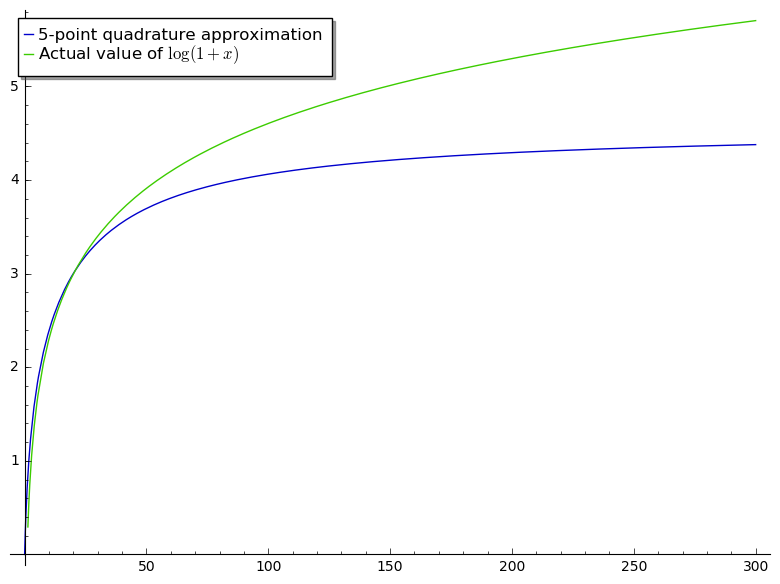
\includegraphics[width=.7\linewidth,\keepaspectratio]{figures/StandardQuadrature.png}
    \caption{Graph of $\log{(1+x)}$ and the approximation in equation \ref{eq:standardquadrature}}
    \label{fig:standardquadrature}
\end{figure}
As we only need accuracy for $x \in [0, 255]$, we can scale the approximation by a constant factor $\alpha$ as follows:
\begin{align*}
  \log{(1+x)} &= \log{\left(\frac{\alpha + \alpha x}{\alpha}\right)}\\
  &= \log{(\alpha + \alpha x)} - \log{\alpha}\\
  &= \log{\left(\alpha+\frac{\alpha}{n}\right)} - \log{\alpha}\\
  &= \log{\left(\frac{\alpha n + \alpha}{n}\right)} - \log{\alpha}\\
  &= \int_{n}^{\alpha n + \alpha}{\frac{1}{x}\diff x} - \log{\alpha}
\end{align*}

Using the five-point Gauss-Legendre quadrature rule with $\alpha = 1/20$, we arrive at the approximation:
\begin{align}\label{eq:scaledquadrature}
  \begin{split}
    &\log(1+x) \\
    &=\frac{137x^5 + 33185x^4 + 931370x^3 - 13403630x^2 - 289469315x - 713567363}
    {30(x^5 + 505x^4 + 42010x^3 + 923010x^2 + 5722005x + 8040501)} + \log{20}
  \end{split}
\end{align}
Below is a graph of the absolute error of the scaled approximation and the exact value of $\log{(1+x)}$.
\begin{figure}[!ht]
    \centering
    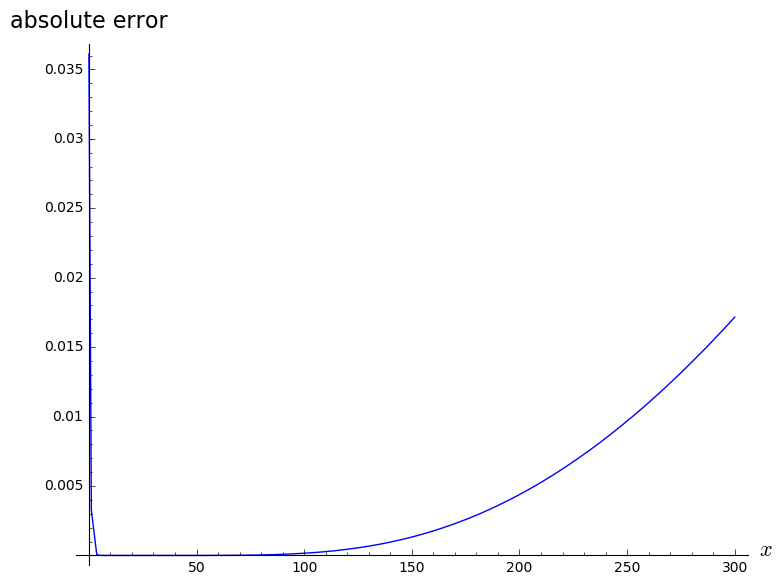
\includegraphics[width=.9\linewidth,\keepaspectratio]{figures/ModifiedQuadratureAbsoluteError.png}
    \caption{Graph of the absolute error of $\log{(1+x)}$ and the approximation in equation \ref{eq:scaledquadrature}}
    \label{fig:scaledquadrature}
\end{figure}
\section{Approximation for $x^\gamma$}
To approximate $x^\gamma$ for any $\gamma \in \mathbb{R}$, we rewrite $x^\gamma$ as follows:
\begin{align*}
  x^\gamma = e^{\log{x^\gamma}} = e^{\gamma\log{x}}.
\end{align*}
This expression can then be approximated using the Maclaurin series expansion for $e^x$, which converges for all $x$.
\begin{align*}
  e^x &= \sum_{n=0}^{\infty}{\frac{x^n}{n!}}\\
  \Rightarrow e^{\gamma\log{x}} &= \sum_{n=0}^{\infty}{\frac{(\gamma\log{x})^n}{n!}}
\end{align*}
As we already have an approximation for the natural logarithm, we can evaluate partial sums of the above infinite series to arrive at approximations for $x^\gamma$.

\end{appendices}


\end{document}
